% For formatting purposes only 
\setcounter{chapter}{8}
\setcounter{section}{3}
\setcounter{subsection}{0}
%\listofalgorithms - think about it ...
%--------------
%- COPY START -
%--------------
\paragraph{Idea:} There is  a need for \emph{fast trajectory approximation} method. The basic idea is taken from pilot steering an plane. The pilot is issued a commands from an navigator in very short and precise manner. The movement has its primitive phase when steering is static and its transition phase when steering is moving from one static position to another. 

Imagine having vertical and horizontal flaps on airplane (fig. \ref{fig:movementsExample}). The \emph{navigator} is issuing a command every second to a pilot. Each command is translated by hands of the pilot to an input signal (blue line). The command validity period (black frame) is split into \emph{transition period} (red frame) when input signal is changing and primitive period (magenta frame) when the position of input signal is static.
 
\begin{figure}[H]
    \centering
    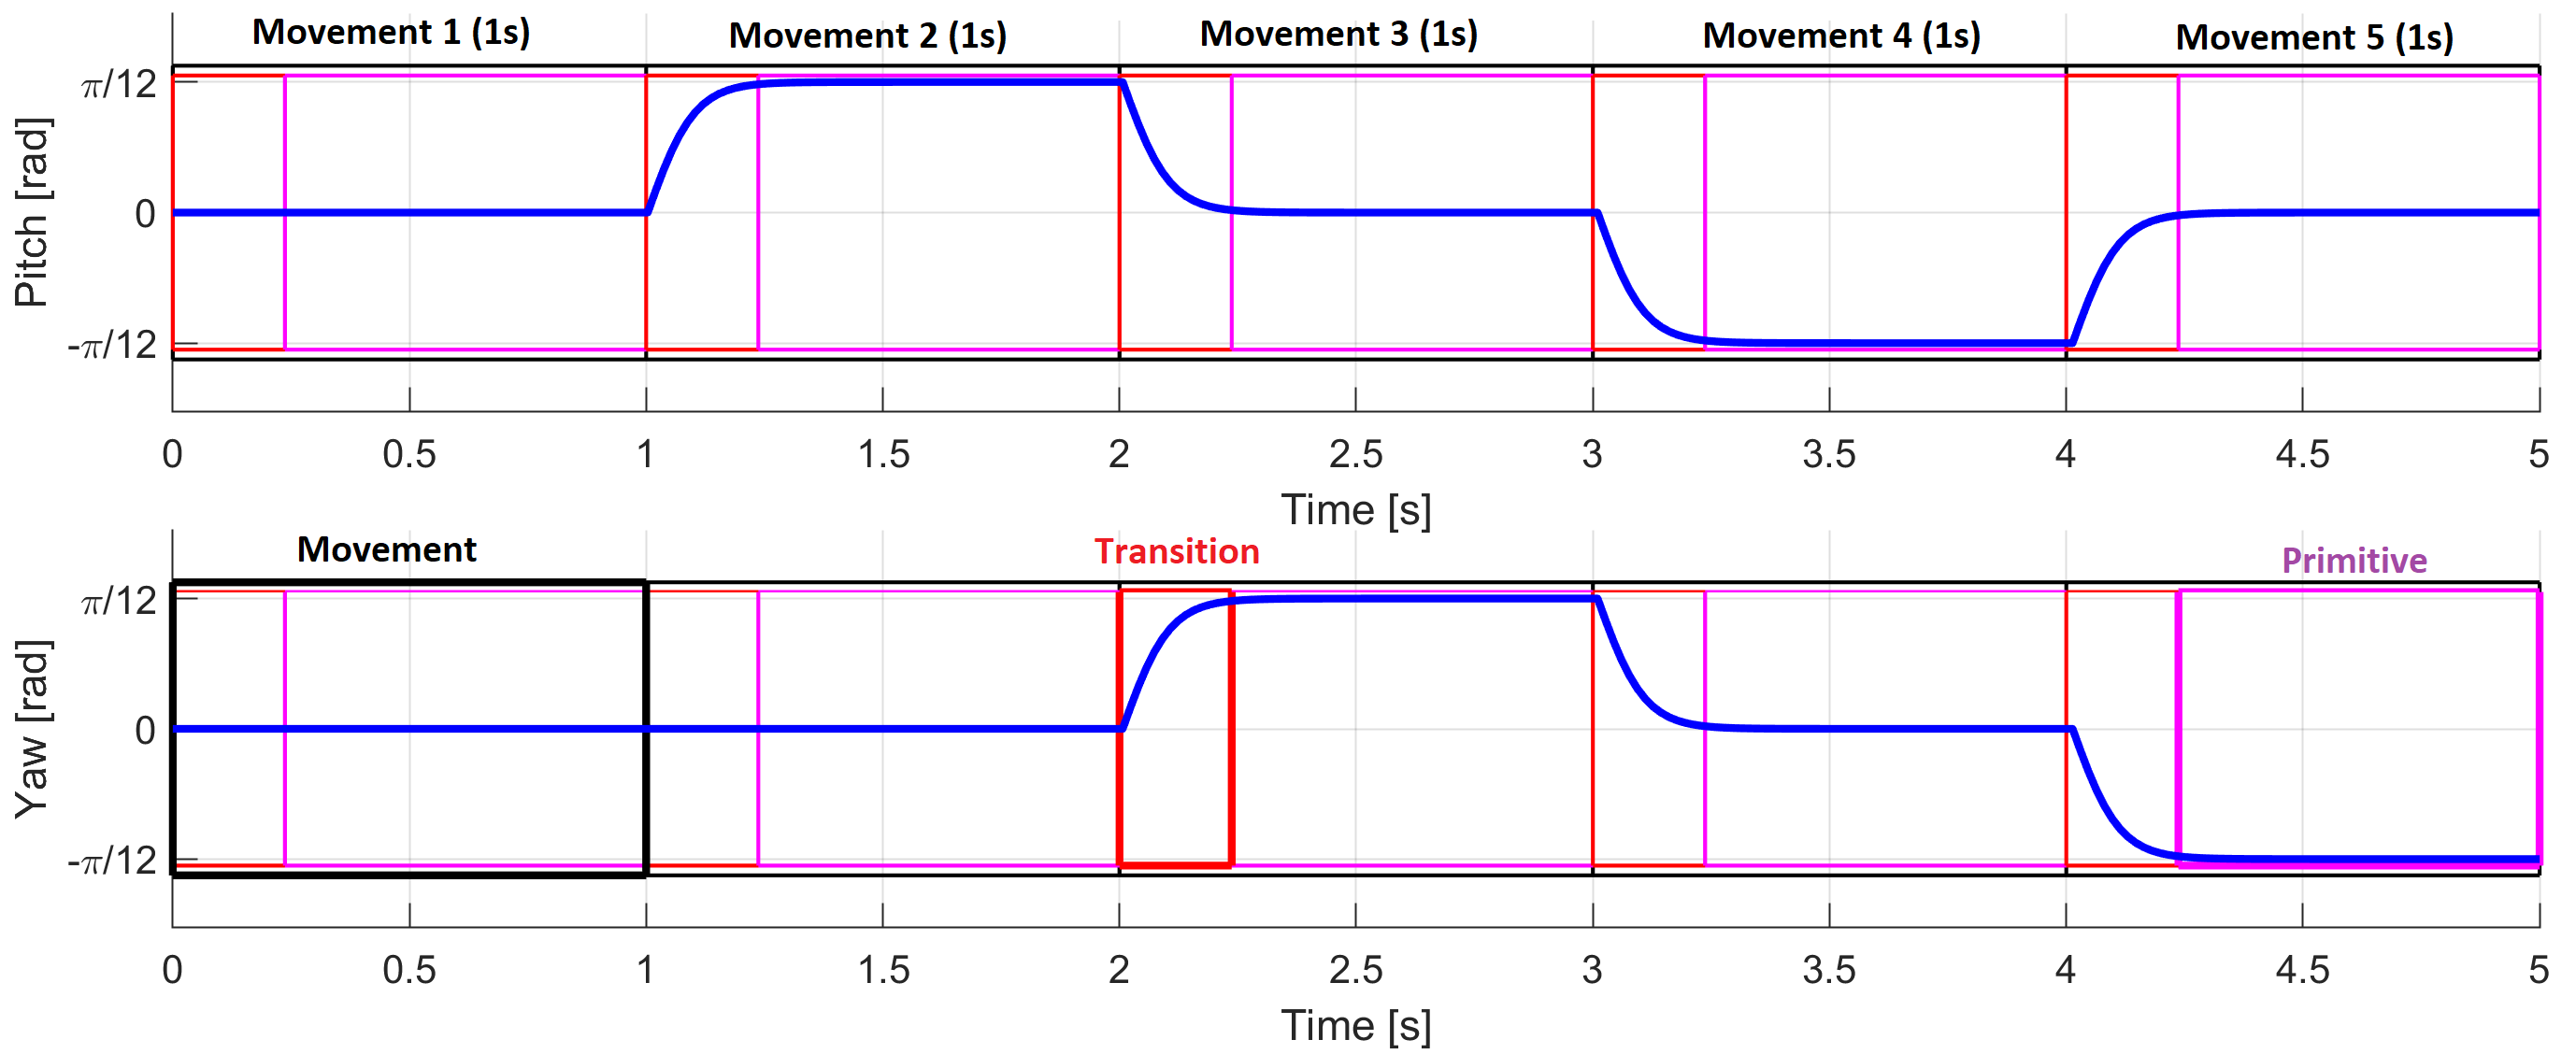
\includegraphics[width=0.95\linewidth]{\FIGDIR/TE062MovementAutomatonExampleWide} 
    \caption{Example of input signal segmentation to movements.}
    \label{fig:movementsExample}
\end{figure}

\begin{note}
    The hybrid automaton (sec. \ref{s:HybridAutomaton}) can be used as the base for simple control mechanism imitating navigators command execution by pilot. The automaton states can be mapped to primitives and transitions. The reset map needs to be replaced with external order issuer to ensure smooth execution of commands.
    
    The future commands will be stacked in the buffer from which they will be picked for an execution.
\end{note}